\chapter{Maßtheoretische Relaxierung}
\textit{Quelle für Definitionen/Sätze dieses Kapitels: \cite{CalcVarBSchmidt}[Seite 103 ff.]}\\[0.1cm]
Wenn man die Variationsrechnung ohne jegliche Einschränkungen/Bedingungen verlässt, kommt man relativ schnell in eine Situation, in der die Maßtheorie eine wichtige Rolle spielt. Betrachtet man beispielsweise die bekannten Euler-Lagrange-Gleichungen für sogenannte Hindernis-Probleme (Englisch: Obstacle-problems), so bekommt man unter gewissen Umständen große Probleme mit "Standard"-Sobolev-Theorie. Betrachten wir nämlich ein Funktional erster Ordnung mit messbarem Integranten (für die, die etwas der geometrischen Maßtheorie vertraut sind: es reicht hier natürlich, einen Caratheodory-Integranden zu fordern, da der Satz von Scorza-Dragoni direkt die\\ \(\mathcal{B}(\mathbb{R}^n) \otimes \mathcal{B}(\mathbb{R}^n)-\)Messbarkeit impliziert (aufgrund der Stetigkeit) und für eine passende monotone Mengenfolge auch die \(\mathcal{M}^n \otimes \mathcal{B}(\mathbb{R}^n)-\)Messbarkeit.) \\ \(F:\mathbb{R}^n \stackrel{offen}{\supset} \Omega \times \mathbb{R}^N \times \mathbb{R}^{N \times n} \to \overline{\mathbb{R}}\), i.e.
\begin{equation}
    \mathcal{F} \in W^{1,1}(\Omega,\, \overline{\mathbb{R}}),\,\mathcal{F}[w] := \int_{\Omega} F(\cdot,w,Dw)\,dx, \, w \in W^{1,p}_{\text{loc}} (\Omega, \mathbb{R}^N)
\end{equation}
Im Falle \(p > n\) können wir mit die Euler-Lagrange-Gleichungen in nur leicht modifizierter Version verwenden, der Fall \(p \le n\) ist allerdings alles andere als trivial. Hier schlägt die Sobolev-Einbettung in den Funktionenraum der stetigen Funktionen fehl auf der Kontaktmenge von Funktional und Hindernis. Wir haben keinerlei stetige Repräsentanten (man benutzt dann Lebesgue-Repräsentanten) und das Lebesgue-Maß ist viel zu stark für "dünne" Hindernisse (Beispiel: Charakteristische Funktion). Dies führt zur Einführung von neuen, geeigneteren Maßen; in diesem Fall die sogenannte Sobolev-p-Kapazität, ein spezielles äußeres Maß. Für mehr zu diesem Thema verweisen wir auf \cite{CalcVar}[Seite 52-69].\\

\begin{figure}[!h]
    \centering
    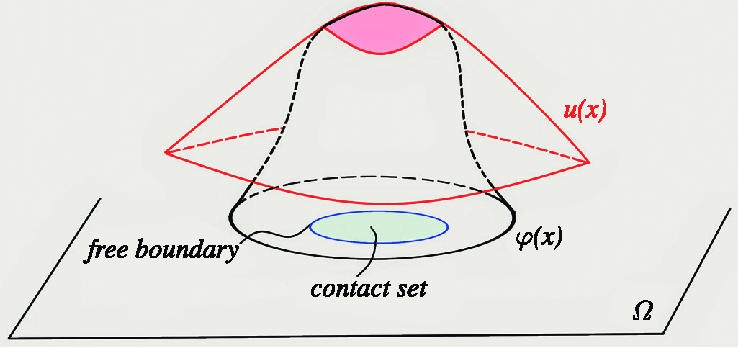
\includegraphics[scale=0.4]{figures/Example-of-an-obstacle-problem.png}
    \caption{Illustrierung eines Hindernis-Problems: Eine ellastische Membran u(x) wird über ein Hindernis \(\varphi(x)\) gespannt; in pink ist die Kontaktmenge dargestellt; diese wird durch eine Karte (in grün-blau) in \(\Omega\) dann dargestellt. \cite{ObstacleProblem}}
    \label{fig:obs}
\end{figure}

Wir werden uns im Folgenden einen Zugang zur Relaxierung mittels Young-Maße schaffen. Doch zunächst sollten wir kurz für das Folgende wichtige Definitionen/Notationen aus der Maßtheorie wiederholen/einführen:\\
\pgfsetfillopacity{0.2}\colorbox{defblue}{\begin{minipage}{16cm}{\textcolor{black}{\pgfsetfillopacity{1}}{\label{def3.1}}}
\textbf{Definition/Notation 3.1:} 
\begin{itemize}
    \item \(\mathcal{C}_0(\mathbb{R}^n) := \overline{\mathcal{C}_c(\mathbb{R}^n)}^{||\cdot||_{\infty}}\).
    \item Sei \(\mathcal{M}^n\) die \(\sigma-\)Algebra aller messbaren Teilmengen \(\Omega\) des \(\mathbb{R}^n\). Der zugehörige Raum ist dann der Banachraum \((\mathcal{M}(\mathbb{R}^n),||\cdot||_{\text{TV}})\) als mit der Totalvariationsnorm normierter Raum aller endlichen signierten Borelmaße auf \(\mathbb{R}^n\). Wir schreiben im Folgenden dann für diesen Raum kurz \(\mathcal{M}(\mathbb{R}^n)\). Hierbei ist die Totalvariationsnorm definiert als
    \begin{equation}
        ||\mu||_{\text{TV}} := \mu^+(\Omega) + \mu^-(\Omega)\, \, \forall \mu \in \mathcal{M}(\mathbb{R}^n),
    \end{equation}
    indem wir \(\mu = \mu^+ - \mu^-\) aus dem Zerlegungssatz von Jordan (siehe Anhang) erhalten.
    \item \(L^{\infty}_{w^*}(\Omega,\,\mathcal{M}(\mathbb{R}^n))\) bezeichnet den Funktionenraum (von Äquivalenzklassen von) schwach*-messbaren, wesentlich beschränkten Funktionen für i.A. \(\Omega \stackrel{messbar}{\subset} \mathbb{R}^n\).
    \item Für allgemeinere Abbildungen \(f:\Omega \to \mathcal{B}\), mit \(\mathcal{B}\) einem Banachraum, definieren wir analog zum Lebesgue-Integral das sogenannte Bochner-Integral auf einem \(\sigma-\)endlichen und vollständigen Maßraum \((\Omega,\Sigma_{\Omega},\mu)\) durch:
    \begin{equation}
        \forall \text{ disjunkten } B_i \in \Sigma_{\Omega}: \int_{\Omega} f \, d\mu := \int_{\Omega} (\sum_{i=1}^n \chi_{B_i}x_i) d\mu := \sum_{i=1}^n \mu(B_i)x_i,
    \end{equation}
\end{itemize}
\end{minipage}}

\begin{figure}[!h]
    \centering
    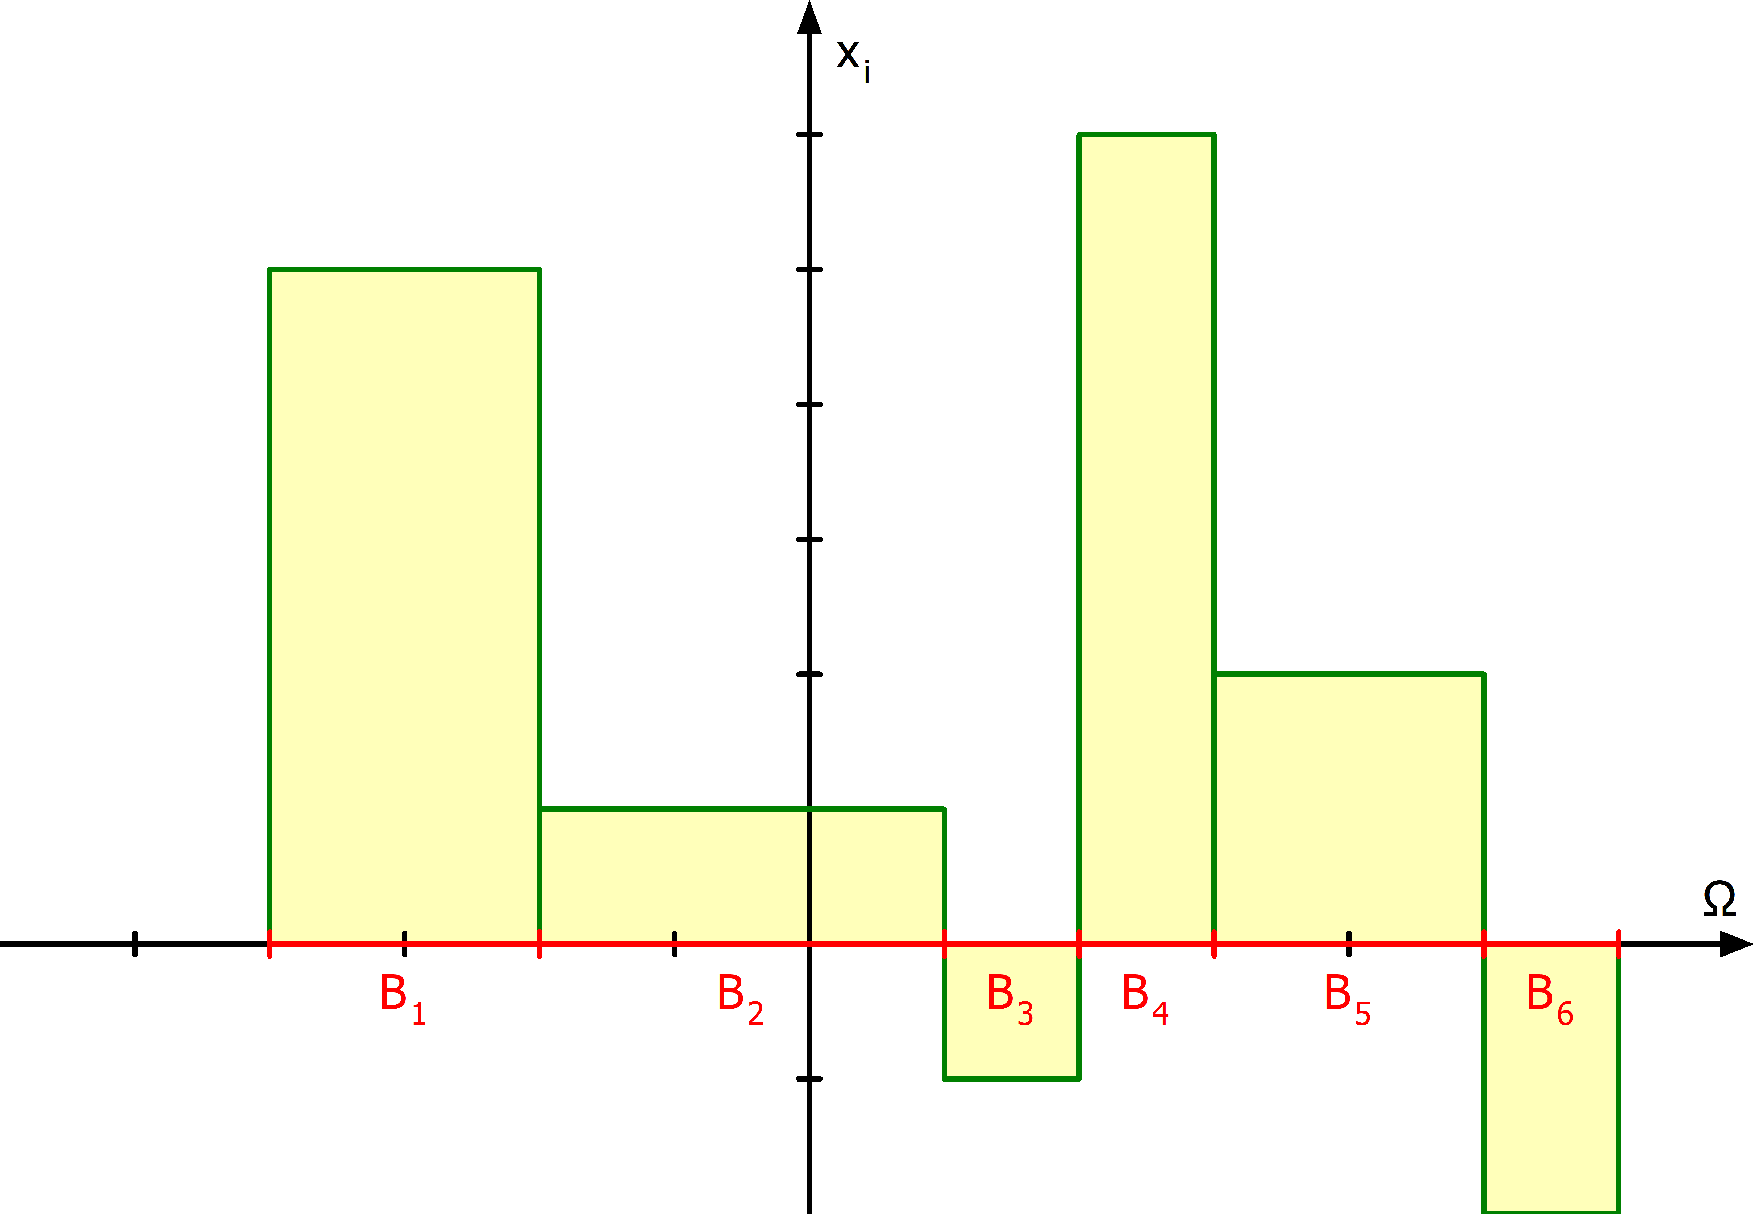
\includegraphics[scale=0.4]{figures/BochnerOhneUrsprungPDF.pdf}
    \caption{Illustration des Bochner-Integrals}
    \label{fig:boch}
\end{figure}

Wir geben nun zwei sehr interessante Resultate für Young-Maße an, von dem eines für die abschließende Betrachtung des Bolza-Problems (1.5) von großer Bedeutung sein wird. Jedoch werden wir aus Zeitgründen diese Resultate nicht beweisen, verweisen für die (nicht uninteressanten) Beweise auf \cite{CalcVarBSchmidt}[Seite 106-109].\\
\pgfsetfillopacity{0.2}\colorbox{theored}{\begin{minipage}{16cm}{\textcolor{black}{\pgfsetfillopacity{1}}{\label{theo3.2}}}
\textbf{Satz 3.2 (Hauptsatz für Young-Maße):} Betrachte \(\Omega \stackrel{messbar}{\subset} \mathbb{R}^n\) und eine messbare Funktionenfolge \(w_k:\Omega \to \mathbb{R}^n\). Dann \(\exists\) Teilfolge \(w_{k_j}\) von \(w_k\), \(\nu \in L^{\infty}_{w^*}(\Omega,\,\mathcal{M}(\mathbb{R}^n))\), sodass gilt:
\begin{enumerate}
    \item \begin{equation}
        \nu_x \geq 0\, \land ||\nu||_{\mathcal{M}(\mathbb{R}^n)} = \int_{\mathbb{R}^n} d\nu_x \le 1\text{ f.f.a. x}
    \end{equation}
    \item \begin{equation}
        \forall f \in \mathcal{C}_0(\mathbb{R}^n):\, f(w_{k_j}) \stackrel{*}{\rightharpoonup} \,<\nu_x,f> \,:= \int_{\mathbb{R}^n} f(y)\,d\nu_x(y)\text{ in }L^{\infty}(\Omega,\,\mathbb{R}^d).
    \end{equation}
\end{enumerate}
\end{minipage}}\\

Das hier erzeugte Maß \(\nu\) erweckt den Eindruck durch die Charakterisierung dieses Hauptsatzes, dass es ein Wahrscheinlichkeitsmaß beschreibt. Und tatsächlich kann man genau das auch zeigen. Benannt wird dieses Maß nach Laurence Chisholm Young, der dieses gefunden hatte:\\
\pgfsetfillopacity{0.2}\colorbox{defblue}{\begin{minipage}{16cm}{\textcolor{black}{\pgfsetfillopacity{1}}{\label{def3.3}}}
\textbf{Definition 3.3 (Young-Maß):} Betrachte eine Familie von Maßen \(\nu := (\nu_x)_{x \in \Omega}\) und eine messbare Funktionenfolge \(w_k:\Omega \to \mathbb{R}^n\). Dann nennen wir die Abbildung
    \begin{equation}
        \nu: \Omega \to \mathcal{M}(\mathbb{R}^n)
    \end{equation}
    das von \(w_{k_j}\) (als Teilfolge von den \(w_k\)) erzeugte Young-Maß.
\end{minipage}}\\

Das Young-Maß ist ziemlich gut reguliert. So trägt es z.B. die starke Regularitäts-Eigenschaft, dass Maß-Konvergenz auf einer kompakten Teilmenge des \(\mathbb{R}^n\) impliziert, dass diese kompakte Menge schon den gesamten Träger des Maßes beinhaltet:\\
\pgfsetfillopacity{0.2}\colorbox{theored}{\begin{minipage}{16cm}{\textcolor{black}{\pgfsetfillopacity{1}}{\label{theo3.4}}}
\textbf{Satz 3.4 (Eigenschaft von Young-Maßen):} Betrachte die gleichen Voraussetzungen wie in [\ref{theo3.2}][Satz 3.2]. Sei zudem \(K \subset \mathbb{R}^n\) kompakt. Dann gilt:
\begin{equation}
    \text{dist}(w_{k_j},K) \stackrel{\nu}{\to} 0 \, \Rightarrow \, \text{supp }\nu_x \subset K\text{ f.f.a. x}.
\end{equation}
\end{minipage}}\\

Wir befinden uns nun in der Situation, in der wir eine maßtheoretische Lösung für die Relaxierung des Bolza-Problems (1.5) beschreiben können. Hierzu betrachten wir der Einfachkeit wegen (1.5) mit a=0, b=1.\\
Betrachte also eine Minimierungsfolge \(u_k\), i.e. \(w_k := u'_k\). Die Voraussetzungen von [\ref{theo3.2}][Satz 3.2] sind erfüllt, also existiert zunächst einmal eine Teilfolge \(w_{k_j}\), die ein Young-Maß \(\nu\) erzeugt. Die Folge \(w_k\) ist beschränkt in \(L^4(]0,1[)\) (Definition Minimierungsfolge), also gilt \(||\nu_x||_{\mathcal{M}(\mathbb{R}^n)} = 1\) (für einen Beweis siehe: \cite{CalcVarBSchmidt}[Seite 106, Bemerkung 3]). Wir wählen für ein \(\epsilon > 0\) nun ein \(\delta > 0\), sodass
\begin{equation}
    (x^2 - 1)^2 < \delta \, \Rightarrow \, \min \{|x-1|,\,|x+1|\} < \epsilon
\end{equation}
gilt. Es folgt:
\begin{equation}
    |\{\text{dist}(w_{k_j},\{-1,1\})\geq \epsilon\}| \le |\{(w^2_{k_j} - 1)^2 \geq \delta\}| \le \frac{1}{\delta} \int_{0}^1 (w^2_{k_j} - 1)^2 \, dx \le \frac{1}{\delta}\mathcal{F}(u_{k_j}) \stackrel{j \to \infty}{\to} 0
\end{equation}
Mit [\ref{theo3.4}][Satz 3.4] folgt supp \(\nu_x \subset \{-1,1\}\) f.f.a. x. Es gilt also:
\begin{equation}
    \exists \lambda(x) \in [0,1]:\,\nu_x = \lambda(x)\delta_{-1} + (1-\lambda(x))\delta_1,
\end{equation}
wobei \(\delta_{(\cdot)}\) das Dirac-Maß bezeichnet. Zudem ist:
\begin{enumerate}
    \item \(u'_{k_j} = w_{k_j} \rightharpoonup w\text{ in }L^4(]0,1[)\)
    \item \(w(x) := \,<\nu_x,id>\, = 1-2\lambda(x)\)
    \item \(\forall \varphi \in \mathcal{C}^{\infty}_c(]0,1[):\, \int_{[0,1]} w\varphi\,dx = \lim_{j \to \infty} \int_{[0,1]} w_{k_j} \varphi\,dx \stackrel{P.I.}{=} 0\)
\end{enumerate}
Für einen Beweis von (1) verweisen wir auf \cite{CalcVarBSchmidt}[Seite 106, Bemerkung 4] (modifizierte Variante von Banach-Alaoglu). Also muss \(w \equiv 0\) gelten (Fundamentallemma) f.ü. und damit ist \(\lambda(x) = \frac{1}{2}\) f.ü. Damit haben wir gezeigt, dass \(w_{k_j}\) das Young-Maß
\begin{equation}
    \nu_x = \frac{1}{2}(\delta_{-1} + \delta_1)\,\,\text{ f.f.a. x}
\end{equation}
erzeugt.\\

Die abschließende Frage ist nun natürlich: Wie hängen das Young-Maß und die Relaxierung von Integralfunktionalen zusammen? Die Antwort ist die Folgende:\\
\pgfsetfillopacity{0.2}\colorbox{theored}{\begin{minipage}{16cm}{\textcolor{black}{\pgfsetfillopacity{1}}{\label{theo3.5}}}
\textbf{Satz 3.5 (Young-Maße und Integralfunktionale):} Sei \(w_k: \Omega \to \mathbb{R}^n\) eine messbare Funktionenfolge, dessen Teilfolge \(w_{k_j}\) das Young-Maß \(\nu\) generiert, \(f \in \mathcal{C}^0(\Omega \times \mathbb{R}^n)\) eine nach unten beschränkte Funktion. Dann gilt:
\begin{enumerate}
    \item \begin{equation}
        \liminf_{k \to \infty} \int_{\Omega} f(x,w_k(x))\,dx \geq \int_{\Omega} \int_{\mathbb{R}^n} f(x,y)\,d\nu_x(y)\,dx
    \end{equation}
    \item Ist zudem \(f(\cdot,w_k(\cdot))\) schwach relativ folgenkompakt in \(L^1(\Omega)\), gilt:
    \begin{equation}
        f(\cdot,w_k) \rightharpoonup \, <\nu_x,f>.
    \end{equation}
\end{enumerate}
\end{minipage}}